\documentclass{article}
\usepackage[spanish]{babel}   
\usepackage[numbers,sort&compress]{natbib}
\usepackage{float}
\usepackage{listings}
\usepackage{graphicx} 	% Nos permite importar imagenes 
\usepackage{subcaption}
\usepackage[left=3cm,right=3cm,top=3cm,bottom=3cm]{geometry}


\usepackage{amssymb}% Símbolos extra



%-------------------------- Por si se romple la URL --------------------------
\usepackage[hyphens]{url}
\usepackage[hidelinks]{hyperref}
\hypersetup{breaklinks=true}	
\urlstyle{same}
\usepackage{cite}
%-------------------------- Por si se romple la URL --------------------------

\title{Reporte Tarea 5}
\author{Victor Alejandro Oviedo Martínez}



\begin{document}
\maketitle
\hrule

\section{Introduccón}\label{intro}
Para esta quinta tarea\citep{DRA.P5} se ha estudiado el tema método Monte-Carlo, el cual, utiliza las probabilidades del sistema para realizar aproximaciones al  resultado deseado.\\

Cómo caso de estudio se realizó el cálculo para la siguiente integral definida:   

\begin{equation}
\label{eq:e1}
\int_{3}^{7}  \! f(x) \, dx  ~ , ~~~~~ f(x)= \frac{1}{e^x + e^{-x}} 
\end{equation}

\begin{equation}
\label{eq:e2}
 g(x) = \frac{2}{\pi}  f(x) 
 \end{equation}

\begin{equation}
\label{eq:e3}
\int_{-\infty}^{\infty}  \! \frac{2}{\pi}  f(x) \, dx = 1
\end{equation}

\begin{equation}
\label{eq:e4}
 \int_{3}^{7}  \! g(x) \, dx  ~~~~  \therefore ~~~~   \frac{2}{\pi} \left(\int_{3}^{7}  \! g(x) \, dx  \right) ~~ = ~~ \int_{3}^{7}  \! f(x) \, dx
\end{equation}
\\

Dada la función $f(x)$ se pretende obtener su integral definida desde 3, hasta 7 (\ref{eq:e1}). Integrando $f(x)$ desde $-\infty$ hasta $\infty$  se tiene que esta no cuenta con una distribución valida, afortunadamente $g(x)$ si cuenta con una distribución valida (\ref{eq:e2})(\ref{eq:e3}), por lo tanto, se evaluará $g(x)$ y sus resultados serán normalizados para obtener la respuesta de la integral definida de $f(x)$.\\




 
 


\section{Desarrollo}
Para esta quinta tarea se ha planteado el siguiente problema: Determina el tamaño de muestra requerido por cada lugar decimal de precisión del estimado obtenido para el integral, comparando con Wolfram Alpha para por lo menos desde uno hasta siete decimales; representa el resultado como una sola gráfica o de tipo caja-bigote o un diagrama de violin. Alternativamente, o en adición, puedes aplicar un método Monte Carlo para estimar la cantidad de pintura necesaria en un mural, comparando conteos exactos de pixeles de distintos colores (recomiendo discretizar a un palette de pocos colores) con conteos estimados con muestreo aleatorio. Completando ambas opciones permite puntajes hasta ocho en la tarea base.


	\subsection{Intento 1}
 Para el desarrollo de este primer intento de la  tarea se a utilizado el código ejemplo proporcionado por \citet{DRA.Code} , el cual tiene el propósito de calcular la integral definida explicada en la introducción. Esté código será  tomando como base y modificando para las características de esta tarea.\\ 
 
 \textbf{Objetivo}.- Determina el tamaño de muestra requerido por cada lugar decimal de precisión del estimado obtenido para el integral, comparando con Wolfram Alpha para por lo menos desde uno hasta siete decimales.\\
 
 La edición de este código empieza tratando de idear alguna forma de poder comparar dos números decimal por decimal. Dado que el programa base de Schaeffer ya entrega el estimado de la integral, podremos comparar  estos dos valores. Por lo tanto, se crea la variable \texttt{wolf} la cual tendrá el valor calculado de Wolfram en formato \textit{string} con la finalidad de poder comparar cada carácter, de igual forma se guarda el resultado del calculo de la integral para su posterior comparación. Para el proceso de comparación se tiene, dos variables en formato \textit{string} las cuales gracias a este formato podemos pedir la comparación de cualquier carácter, por lo tanto, se podría iterar el programa aumentando cada vez la variable \texttt{pedazo} y observar en que valor de \texttt{pedazo} se cumple la igualdad para cada decimal. A continuación, se podrá observar la forma en la cual se pretende realizar la comparación de decimales.
 
 \begin{lstlisting}[language=Python]
        
while (True):
            montecarlo = pool.map(parte, range(cuantos))

            integral = sum(montecarlo) / (cuantos * pedazo)
            num = str((pi / 2) * integral)
            pedazo = pedazo + 100


            if num[0] == wolf[0] and num[1] == wolf[1] and num[2] == wolf[2]
             and state == 0: # 1er Decimal
                                state = 1

            if num[0] == wolf[0] and num[1] == wolf[1] and num[2] == wolf[2]
             and num[3] == wolf[3] and state == 1: # 2do Decimal
                                state = 2
                                
                                          *
                                          *
                                          *
                                          
            if num[0] == wolf[0] and num[1] == wolf[1] and num[2] == wolf[2]
             and num[3] == wolf[3] and num[4] == wolf[4] and num[5] == wolf[5]
             and num[6] == wolf[6] and num[7] == wolf[7] and num[8] == wolf[8] 
             and state == 6: # 7mo Decimal
                break            
 \end{lstlisting}
 
 Cómo se pudo observar, primero tenemos el bucle \texttt[while] con el fin de repetir el calculo indefinidamente hasta que se logren los 7 decimales, al cumplirse los 7 decimales el programa se detendrá gracias al comando \texttt{break} al final de todos los \texttt{if}. En total se tendrán 7 diferentes \texttt{if} uno para cada decimal, ademas de la comparación de cada decimal se ha agregado la variable \texttt{state} con el fin de no repetir decimales ya evaluados.\\
 
Hasta este punto, se tiene que la lógica de comparación de decimales funciona de manera correcta. Para esta tarea se ha pedido encontrar el tamaño de muestra requerido para lograr 7 decimales de precisión, se pensaba que esto no era posible por culpa de la receta, sin embargo, una vez analizado el programa se pudo observar que el problema estaba en el tamaño del arreglo para la variable \texttt{X}, ya que el vector que generaría los valores de \texttt{X} no era lo suficiente mente fino, por lo tanto, se modifico el valor de 0.01 a 0.001, con esto reduciremos el error por la estimación del área por debajo de la curva. Es importante mencionar que hay que tener cuidado con la este valor, ya que de hacerlo muy fino todos los valores a generar tardaran mucho aunque este no contenga gran cantidad de números e iteraciones. \\

Una vez solucionado el problema con la limitante que se tenia con la receta, se observo que al momento de ejecutar el programa los valores entregados no eran correctos, ya que a medida que se iteraba el program los resultados eran cada vez mas erróneos. Revisando el código se llego a la conclusión que el error se generaba en algún lugar de la receta, ya que este tipo de errores en donde cada vez que iteras se agudiza el error se presentan por valores acumulados de iteraciones pasadas, sin embargo el programa fue revisado y desafortunadamente no se  encontró el error. 
  
  \subsubsection{Conclusión}
Esta parte de la tarea no fue posible terminarla por el inconveniente con el error de iteración, en el cual al realizar la primera iteración se tiene un valor correcto, sin embargo, al seguir realizado mas iteraciones se genera  un error el cual aumentaba a medida que se sigue iterando. Se cree que el problema puede estar dentro de la receta, se intentó resolver el problema pero no se tiene el conocimiento suficiente con la estructura de las clases. De resolver este problema el program podría cumplir con el objetivo de la tarea.


\subsection{Intento 2}
\textbf{Objetivo}.- Aplica un método Monte Carlo para estimar la cantidad de pintura necesaria en un mural, comparando conteos exactos de pixeles de distintos colores (recomiendo discretizar a un palette de pocos colores) con conteos estimados con muestreo aleatorio.\\

Para el desarrollo de este código se inició eligiendo una imágen pequeña y de pocos colores con el fin de no tardar tanto al momento de su procesamiento figura \ref{fig:cuadro.1}. \\

\begin{figure}[H]
\begin{center}
	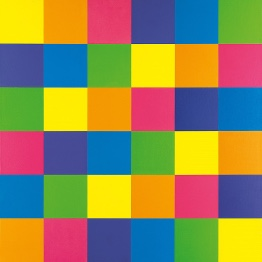
\includegraphics[height=2.65in]{/Users/victor/Desktop/colores.jpg}
	\caption{ Imagen a utilizar (colores.jpg).}
	\label{fig:cuadro.1}
\end{center}
\end{figure}

Una vez elegida la imagen se procede a importar la figura \ref{fig:cuadro.1}. Para la manipulación de imagenes se utiliza la librería \texttt{PIL} . A continuación, se tendrá parte del programa:  


\begin{lstlisting}[language=Python]
        try:
    Imagen = Image.open("colores.jpg")

except IOError:
    print("Unable to load image")
    sys.exit(1)


size = w, h = Imagen.size
data = Imagen.load()

total_pixel = w * h

print("\nLa imagen a porcesar tiene las siguientes caracteristicas:\n")
print(" Format: {0}\n Size: {1}\n Mode: {2}".format(Imagen.format,
    Imagen.size, Imagen.mode), "\n")


print("Por lo tanto, para esta imagen se tiene un total de", total_pixel, 
"pixeles.\n")

 \end{lstlisting}
 
 
Cómo se pudo ver en el código anterior, se tiene el procedimiento para la importación de la imagen seleccionada , así como la obtención de algunos parámetros de interés. Después se tiene el código para la lectura de todos los pixeles de la imagen. Cada vez que se obtenga el color de un pixel el programa obtendrá la cantidad de pintura que se necesitará de cada color (\texttt{RGB}), estos valores serán almacenados hasta haber pasado por todos los pixeles, por lo tanto, al final obtendremos la cantidad de pintura necesaria para pintar la imagen en litros.\\
 


\begin{lstlisting}[language=Python]
Global_R, Global_G, Global_B = [], [], []

colors = []
for x in range(w):
    for y in range(h):

        colores = data[x,y]
        Ra, Ga, Ba = colores[0], colores[1], colores[2]

        sum_RGB = (Ra + Ga + Ba)
        porcentaje_R = ((Ra * 100)/sum_RGB)
        porcentaje_G = ((Ga * 100)/sum_RGB)
        porcentaje_B = ((Ba * 100)/sum_RGB)
        Lt_R = ((porcentaje_R)/ 100)
        Lt_G = ((porcentaje_G)/ 100)
        Lt_B = ((porcentaje_B)/ 100)
        Global_R.append(Lt_R)
        Global_G.append(Lt_G)
        Global_B.append(Lt_B)



R = sum(Global_R)
G = sum(Global_G)
B = sum(Global_B)
 \end{lstlisting}
 
 Conociendo la cantidad de pintura necesaria para cada  color, se tomaron estos valores como el 100$\%$ de pintura ha utilizar. Por lo tanto, lo siguiente fue generar colores al azar con el fin de comparar la cantidad de pintura faltante para obtener el 100$\%$. A continuación, se podrá observar el código para este resultado:
 
 \begin{lstlisting}[language=Python]
 while (True):
    repeticiones = repeticiones + 1

    r = randint(0, 256)
    g = randint(0, 256)
    b = randint(0, 256)


    sum_rgb = (r + g + b)
    porcentaje_r = ((r * 100)/sum_rgb)
    porcentaje_g = ((g * 100)/sum_rgb)
    porcentaje_b = ((b * 100)/sum_rgb)
    if PORCENTAJES_R <= 100:
        Lt_r = ((porcentaje_r)/ 100)
    else:
        Lt_r = 0
    if PORCENTAJES_G <= 100:
        Lt_g = ((porcentaje_g)/ 100)
    else:
        Lt_g = 0
    if PORCENTAJES_B <= 100:
        Lt_b = ((porcentaje_b)/ 100)
    else:
        Lt_b = 0
    Global_r.append(Lt_r)
    Global_g.append(Lt_g)
    Global_b.append(Lt_b)
    Total_r = sum(Global_r)
    Total_g = sum(Global_g)
    Total_b = sum(Global_b)
    
    PORCENTAJES_R = ((Total_r * 100) / R )
    PORCENTAJES_G = ((Total_g * 100) / G )
    PORCENTAJES_B = ((Total_b * 100) / B )

    grafica_R.append(PORCENTAJES_R)

    grafica_G.append(PORCENTAJES_G)

    grafica_B.append(PORCENTAJES_B)


    if PORCENTAJES_R >= 100 and PORCENTAJES_G >= 100 and PORCENTAJES_B >= 100:
        break
  \end{lstlisting}
 
 Como se pudo observar el código anterior genera 3 diferentes valores, para representar un pixel, luego se calcula el el estimado de pintura para el pixel, luego con esta cantidad de pintura se realiza el estimado para conocer el porcentaje de la pintura para poder ser comparado con el 100$\%$ de la pintura a necesitar. Este procedimiento se realiza hasta que todos los colores alcancen el 100$\%$ de la pintura. Una vez llegado todos los colores al 100$\%$ se realiza la grafica del comportamiento de la simulación. Estos resultados se podrán observar en la figura \ref{fig:cuadro.2}.
 
 
\begin{figure}[H]
\begin{center}
	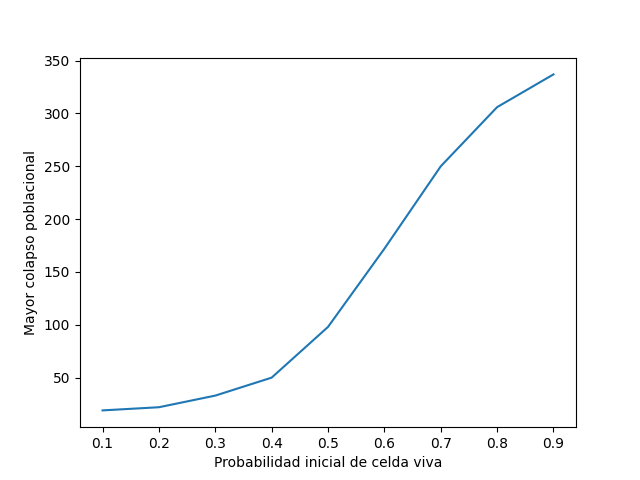
\includegraphics[height=3in]{/Users/victor/Desktop/Figure_1.png}
	\caption{ Resultados de la simulación.}
	\label{fig:cuadro.2}
\end{center}
\end{figure}
 
Para el desarrollo de esta tarea se utilizó la pagina \citep{DRA.Code}.


\subsubsection{Conclusión}
 Para esta parte de la tarea se pudo estimar la cantidad de pintura necesaria para pintar la imagen, sin embargo, no se encontró la manera de implementar el método Monte-Carlo, por lo tanto, el resultado de esta parte de la tarea es el intento fallido  de implementar el método Monte-Carlo para el propósito ya conocido. 









%-------------------------- Por si se rompe la URL --------------------------
\Urlmuskip=0mu plus 1mu\relax
%-------------------------- Por si se rompe la URL --------------------------
\bibliography{ref.Tarea5.bib}
\bibliographystyle{plainnat}

\end{document}